% =====================================================================
\chapter{Capacidades emergentes y contexto largo}
\label{tema:6}
% =====================================================================

Las leyes de escalado predicen bien la pérdida de preentrenamiento. Este tema trata dos cuestiones en las que la escala produce efectos menos regulares. La primera es la aparición aparentemente brusca de capacidades al crecer el modelo, y si esa brusquedad es una propiedad del modelo o de la forma de medir. La segunda es la ampliación de la ventana de contexto, que tropieza con el coste cuadrático de la atención, con la memoria de la caché de claves y valores y con la codificación de posiciones no vistas en el entrenamiento. Se sigue a Wei \emph{et al.}~\cite{wei}, Schaeffer, Miranda y Koyejo~\cite{schaeffer} y la clase «Capabilities» de CS324~\cite{cs324} para la primera parte, y a Chen \emph{et al.}~\cite{chenpi}, el informe de Llama~3~\cite[§3.4.2]{llama3} y Liu \emph{et al.}~\cite{liu} para la segunda; el modelo probabilístico de las respuestas usa la independencia de Bertsekas y Tsitsiklis~\cite[§1.5]{bt}.

\section{Capacidades emergentes}

\begin{definicion}[Capacidad emergente; Wei \emph{et al.}~\cite{wei}]
Una capacidad es \emph{emergente} si no está presente en los modelos pequeños de una familia y sí en los grandes, de modo que no puede predecirse extrapolando el rendimiento de los primeros.
\end{definicion}

Los ejemplos habituales son tareas de aritmética de varias cifras y algunas tareas del conjunto BIG-Bench, en las que la exactitud permanece cerca del azar en varios órdenes de magnitud de cómputo y después sube con rapidez~\cite{wei}. Si fueran saltos genuinos, la planificación de un modelo grande no podría apoyarse en experimentos pequeños, que es justo lo que hacen los temas~\ref{tema:3} a~\ref{tema:5}.

\section{El argumento de la métrica}

Schaeffer, Miranda y Koyejo~\cite{schaeffer} proponen que muchas de esas discontinuidades las crea la métrica. Supóngase que una respuesta tiene $k$ tokens y que el modelo acierta cada uno con probabilidad $p$, de forma independiente~\cite[§1.5]{bt}. La \emph{exactitud exacta} (todo o nada) es la probabilidad de acertar los $k$:
\[
\PP(\text{respuesta correcta})=p^{k}.
\]
Una mejora gradual de $p$ se convierte en un cambio brusco de $p^{k}$ cuando $k$ es grande:
\begin{center}\small
\begin{tabular}{@{}cccccc@{}}
\toprule
$p$ & $0{,}5$ & $0{,}8$ & $0{,}9$ & $0{,}95$ & $0{,}99$ \\
\midrule
$p^{5}$ & $0{,}031$ & $0{,}328$ & $0{,}590$ & $0{,}774$ & $0{,}951$ \\
$p^{10}$ & $0{,}001$ & $0{,}107$ & $0{,}349$ & $0{,}599$ & $0{,}904$ \\
\bottomrule
\end{tabular}
\end{center}
Pasar de $p=0{,}8$ a $p=0{,}95$ lleva la exactitud de $0{,}107$ a $0{,}599$ con $k=10$. En cambio, el número esperado de tokens correctos, $kp$, crece linealmente con~$p$.

La pérdida por token sí sigue una ley de potencia suave en $N$. La proposición siguiente muestra qué forma adopta entonces la exactitud exacta.

\begin{proposicion}[Exactitud exacta bajo una ley de potencia]\label{prop:gompertz}
Supóngase que la pérdida por token de la respuesta es $\ell(N)=(N_1/N)^{\theta}$, con $N_1,\theta>0$, que $p(N)=e^{-\ell(N)}$ y que la respuesta tiene $k$ tokens. Sea $x=\ln N$. Entonces:
\begin{enumerate}
  \item $A(N)=p(N)^{k}=\exp\bigl(-e^{-\theta(x-x_0)}\bigr)$, con $x_0=\ln N_1+(\ln k)/\theta$: una curva de Gompertz en $\ln N$, creciente de $0$ a $1$;
  \item su único punto de inflexión está en $N_0=N_1k^{1/\theta}$, donde $A=1/e$;
  \item en cambio, $-\ln A(N)=k\,\ell(N)$ es una ley de potencia en $N$, una recta en escala log-log.
\end{enumerate}
\end{proposicion}

\begin{proof}
(i) $A=e^{-k\ell}$ y $k\ell=k\,N_1^{\theta}e^{-\theta x}=e^{\ln k+\theta\ln N_1-\theta x}=e^{-\theta(x-x_0)}$. Como $e^{-\theta(x-x_0)}$ decrece de $+\infty$ a~$0$, $A$ crece de~$0$ a~$1$. (ii) Sea $y=e^{-\theta(x-x_0)}$, de modo que $dy/dx=-\theta y$ y $A=e^{-y}$. Entonces $dA/dx=\theta ye^{-y}$ y $d^{2}A/dx^{2}=\theta(dy/dx)(1-y)e^{-y}=-\theta^{2}y(1-y)e^{-y}$, que solo se anula en $y=1$, es decir, en $x=x_0$, y cambia allí de signo. En ese punto $A=e^{-1}$ y $N=e^{x_0}=N_1k^{1/\theta}$. (iii) $-\ln A=k\ell(N)=kN_1^{\theta}N^{-\theta}$.
\end{proof}

La \cref{prop:gompertz} contiene el argumento completo. La capacidad «aparece» en torno a $N_0=N_1k^{1/\theta}$, y el umbral se desplaza hacia modelos mayores cuanto más larga es la respuesta exigida, aunque la mejora por token sea la misma. Con pocos tamaños de modelo y escala lineal en el eje vertical, la curva parece un escalón (\cref{fig:gompertz}); con la métrica continua $-\ln A$, es una recta en escala log-log.

\begin{figure}[h]
\centering
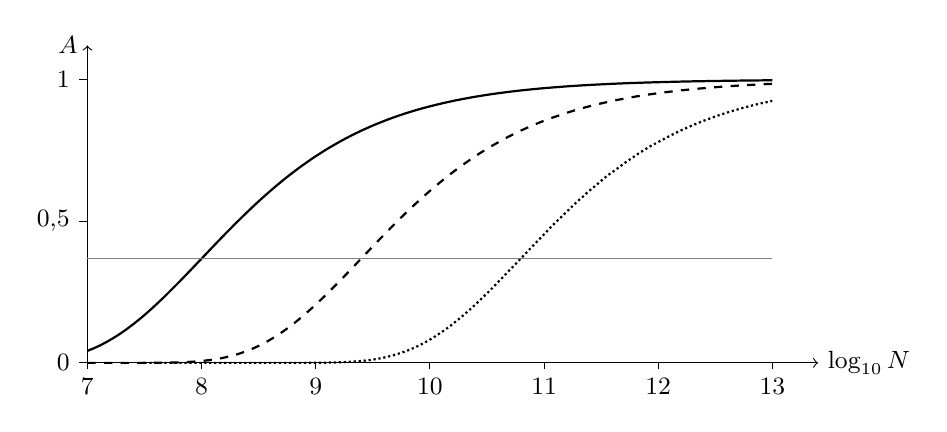
\begin{tikzpicture}[x=1.45cm,y=3.6cm,font=\small]
  \draw[->] (7,0)--(13.4,0) node[right] {$\log_{10}N$};
  \draw[->] (7,0)--(7,1.12) node[left] {$A$};
  \foreach \t in {7,8,...,13} \draw (\t,0)--(\t,-0.02) node[below] {\t};
  \foreach \t in {0,0.5,1} \draw (7,\t)--(6.93,\t) node[left] {\pgfmathprintnumber[use comma]{\t}};
  \draw[thick,domain=7:13,samples=120,smooth] plot (\x,{exp(-1*10^(-(\x-8)/2))});
  \draw[thick,dashed,domain=7:13,samples=120,smooth] plot (\x,{exp(-5*10^(-(\x-8)/2))});
  \draw[thick,densely dotted,domain=7.5:13,samples=120,smooth] plot (\x,{exp(-25*10^(-(\x-8)/2))});
  \draw[gray] (7,0.3679)--(13,0.3679);
\end{tikzpicture}
\caption{Exactitud exacta $A(N)=\exp\bigl(-k(10^{8}/N)^{1/2}\bigr)$ de la \cref{prop:gompertz} para respuestas de $k=1$ (continua), $k=5$ (discontinua) y $k=25$ (punteada) tokens. La línea gris marca $A=1/e$; los puntos de inflexión están en $\log_{10}N_0=8$, $9{,}40$ y $10{,}80$.}
\label{fig:gompertz}
\end{figure}

\begin{observacion}[El debate sigue abierto]
El argumento explica muchas discontinuidades observadas, y Schaeffer \emph{et al.}\ las hacen desaparecer cambiando la métrica o aumentando la resolución estadística~\cite{schaeffer}. No demuestra que no existan cambios cualitativos con la escala: muestra que una curva brusca en una métrica de todo o nada no es, por sí sola, prueba de ellos. Lo que sí está claro es que la pérdida de preentrenamiento es predecible y el rendimiento en una tarea concreta lo es mucho menos.
\end{observacion}

\section{El coste del contexto largo}

La ventana de contexto ha crecido de $2048$ tokens en GPT-3~\cite{brown} a 128K ($131\,072$) en Llama~3~\cite{llama3}; el informe de Gemini~1.5 describe ventanas de millones de tokens, con recuperación casi perfecta hasta al menos $10$ millones, y cita $200\,000$ tokens para Claude~3.0~\cite{gemini15}. Hay tres obstáculos.

\subsection*{Cómputo de la atención}

Por el módulo~14 (tema~6), una pasada hacia delante cuesta por token unos $2N+4L\nctx d$ FLOP, donde $L$ es el número de bloques y $d$ la dimensión del modelo. El segundo término procede de los productos $QK\T$ y $AV$ y crece linealmente con el contexto; sobre una secuencia completa, el coste de la atención crece como $\nctx^{2}$. Pasar de $4096$ a $10^{6}$ tokens multiplica ese término total por $(10^{6}/4096)^{2}\approx 59\,600$.

\begin{ejemplo}\label{ej:atencion-larga}
Para LLaMA-2~7B ($N=6{,}738\cdot 10^{9}$, $L=32$, $d=4096$), el término de atención por token vale $4\cdot 32\cdot 4096\cdot\nctx$. Con $\nctx=4096$ es $2{,}15\cdot 10^{9}$, el $13{,}7\,\%$ del total; con $32\,768$, $1{,}72\cdot 10^{10}$, el $56{,}0\,\%$; con $131\,072$, $6{,}87\cdot 10^{10}$, el $83{,}6\,\%$. A partir de unos $25\,700$ tokens, la atención cuesta más que todas las matrices de pesos juntas. FlashAttention (módulo~17) reduce el tráfico de memoria, pero no el número de operaciones.
\end{ejemplo}

\subsection*{Memoria de la caché KV}

\begin{proposicion}[Tamaño de la caché KV]\label{prop:kv}
Un Transformer de $L$ bloques con $h_{kv}$ cabezas de claves y valores de dimensión $d_k$, que almacena cada número con $\beta_b$ bytes, necesita para una secuencia de $n$ tokens una caché de
\[
M_{KV}=2\,L\,n\,h_{kv}\,d_k\,\beta_b\ \text{bytes}.
\]
\end{proposicion}

\begin{proof}
En cada bloque y para cada token previo se guardan un vector de claves y uno de valores por cabeza, cada uno de $d_k$ números: $2h_{kv}d_k$ números por token y bloque. Se multiplica por $L$ bloques, $n$ tokens y $\beta_b$ bytes por número.
\end{proof}

Para LLaMA-2~7B, con atención multicabeza estándar ($h_{kv}=32$, $d_k=128$) en bf16 ($\beta_b=2$), son $2\cdot 32\cdot 4096\cdot 2=524\,288$ bytes, $0{,}5$ MiB por token: $2$ GiB con $4096$ tokens y $64$ GiB con $131\,072$, más que la memoria de una GPU de $40$ GiB para una sola secuencia. La atención con consultas agrupadas (GQA, módulo~18) reduce $h_{kv}$: con $8$ cabezas de claves y valores, la caché se divide por~$4$. La caché domina el coste de la inferencia con contexto largo (módulo~19).

\section{Posiciones no vistas: interpolación de RoPE}

En RoPE (módulo~14, tema~4), el par de coordenadas $i$ de la consulta y la clave en la posición $m$ se rota un ángulo $m\theta_i$, con $\theta_i=\text{base}^{-2i/d_k}$ para $i=0,\dots,d_k/2-1$, y el producto escalar resultante depende solo de la diferencia de posiciones. Un modelo entrenado con contexto $L_{\mathrm{tr}}$ solo ha visto ángulos en $[0,L_{\mathrm{tr}}\theta_i)$. Para las frecuencias bajas, ese intervalo es una fracción pequeña de una vuelta, y las posiciones $m\ge L_{\mathrm{tr}}$ producen ángulos que el modelo nunca ha visto.

\begin{definicion}[Interpolación de posiciones; Chen \emph{et al.}~\cite{chenpi}]
Sea $L'>L_{\mathrm{tr}}$ el nuevo contexto. La \emph{interpolación de posiciones} sustituye la posición $m$ por $m\,L_{\mathrm{tr}}/L'$ en todas las rotaciones de RoPE, y se ajusta brevemente el modelo con secuencias de longitud $L'$.
\end{definicion}

\begin{proposicion}\label{prop:pi}
Con interpolación de posiciones, para toda posición $0\le m<L'$ y toda frecuencia $i$, el ángulo de rotación está en $[0,L_{\mathrm{tr}}\theta_i)$, el rango visto en el entrenamiento. El producto escalar rotado entre las posiciones $m$ y $n$ sigue dependiendo solo de $m-n$, ahora a través de $(m-n)L_{\mathrm{tr}}/L'$.
\end{proposicion}

\begin{proof}
El ángulo es $\theta_i\,mL_{\mathrm{tr}}/L'$, y $0\le mL_{\mathrm{tr}}/L'<L'L_{\mathrm{tr}}/L'=L_{\mathrm{tr}}$. Para la segunda afirmación, RoPE aplicado a posiciones reales $\mu$ y $\nu$ da un producto escalar que depende solo de $\mu-\nu$ (módulo~14, tema~4); con $\mu=mL_{\mathrm{tr}}/L'$ y $\nu=nL_{\mathrm{tr}}/L'$, $\mu-\nu=(m-n)L_{\mathrm{tr}}/L'$.
\end{proof}

\begin{ejemplo}\label{ej:pi}
Con base $10^{4}$ y $d_k=128$, la frecuencia más baja es $\theta_{63}=10^{-4\cdot 126/128}=1{,}155\cdot 10^{-4}$ rad por posición, con una longitud de onda de $2\pi/\theta_{63}\approx 54\,400$ posiciones. Con $L_{\mathrm{tr}}=2048$, el modelo solo ha visto ángulos hasta $0{,}237$ rad en esa frecuencia; en la posición $32\,768$ el ángulo sería $3{,}78$ rad, nunca visto. Con interpolación, el máximo sigue siendo $0{,}237$. Chen \emph{et al.}\ ampliaron así modelos LLaMA de $7\cdot 10^{9}$ a $65\cdot 10^{9}$ parámetros hasta $32\,768$ tokens con unos $1000$ pasos de ajuste, y obtuvieron una cota del error de la interpolación unas $600$ veces menor que la de la extrapolación~\cite{chenpi}.
\end{ejemplo}

El precio es la resolución: dos posiciones contiguas quedan a $L_{\mathrm{tr}}/L'$ de distancia en lugar de~$1$. Las variantes posteriores reparten el reescalado entre frecuencias (YaRN~\cite{yarn}) o aumentan la base de RoPE; Llama~3 usa base $500\,000$~\cite[§3.2]{llama3}.

\section{La receta habitual y sus límites}

Como el coste de la atención crece con el contexto, casi todo el preentrenamiento se hace con secuencias cortas y se añade una fase final con documentos largos. Llama~3 amplió su ventana de 8K a 128K tokens en seis etapas, con unos $800\,000$ millones de tokens en total~\cite[§3.4.2]{llama3}. Aceptar un contexto largo no equivale a usarlo bien: Liu \emph{et al.}~\cite{liu} observaron que los modelos aprovechan peor la información situada en el centro de un contexto largo que la situada al principio o al final.

\begin{lecturas}
\item Wei \emph{et al.}~\cite{wei} y Schaeffer, Miranda y Koyejo~\cite{schaeffer}.
\item Stanford CS324~\cite{cs324}, clase «Capabilities».
\item Bertsekas y Tsitsiklis~\cite{bt}, §1.5 «Independence» (ensayos independientes).
\item Chen \emph{et al.}~\cite{chenpi}, interpolación de posiciones; Peng \emph{et al.}~\cite{yarn}, YaRN.
\item Dubey \emph{et al.}~\cite{llama3}, §3.4.2 (preentrenamiento con contexto largo); Liu \emph{et al.}~\cite{liu}.
\end{lecturas}

\section*{Ejercicios del tema 6}
\addcontentsline{toc}{section}{Ejercicios del tema 6}

\begin{ejercicio}{1}{eje:6-escepticismo}
Un equipo afirma: «la capacidad~X aparece de golpe a partir de $10^{10}$ parámetros». Enumere tres comprobaciones que haría antes de aceptarlo y justifique cada una.
\end{ejercicio}

\begin{ejercicio}{2}{eje:6-todo-nada}
Una tarea exige generar exactamente una respuesta de $k$ tokens, y el modelo acierta cada token con probabilidad $p$, de forma independiente. (a) ¿Qué $p$ hace falta para una exactitud del $50\,\%$ con $k=10$? ¿Y con $k=20$? (b) Con $k=10$, ¿por qué factor se multiplica la exactitud al pasar de $p=0{,}8$ a $p=0{,}9$? (c) ¿Cuánto cambia, en el mismo paso, el número esperado de tokens correctos?
\fuente{adaptado de Bertsekas y Tsitsiklis~\cite{bt}, §1.5 (probabilidad de que tengan éxito todos los ensayos independientes de una serie).}
\end{ejercicio}

\begin{ejercicio}{2}{eje:6-atencion}
LLaMA~13B tiene $N\approx 1{,}3\cdot 10^{10}$ parámetros, $L=40$ bloques y $d=5120$. (a) ¿A partir de qué contexto el término de atención por token, $4L\nctx d$, supera a $2N$? (b) ¿Qué fracción del coste por token de la pasada hacia delante corresponde a la atención con $\nctx=8192$ y con $\nctx=131\,072$?
\end{ejercicio}

\begin{ejercicio}{2}{eje:6-kv}
Para el modelo del \cref{eje:6-atencion}, con $40$ cabezas de dimensión $d_k=128$ y caché en bf16: (a) calcule la caché KV por token; (b) calcule la caché de una secuencia de $32\,768$ tokens y la de un lote de $8$ secuencias; (c) ¿cuánto ocuparía la de una secuencia si el modelo usara GQA con $8$ cabezas de claves y valores?
\end{ejercicio}

\begin{ejercicio}{3}{eje:6-gompertz}
Con las hipótesis de la \cref{prop:gompertz}, $N_1=10^{8}$ y $\theta=1/2$: (a) calcule $A(N)$ para $k=5$ y $N=10^{8}$, $10^{9}$, $10^{10}$ y $10^{11}$; (b) halle el punto de inflexión para $k=1$, $5$ y $25$ y demuestre que multiplicar $k$ por $\lambda$ desplaza el umbral en $(\log_{10}\lambda)/\theta$ órdenes de magnitud; (c) demuestre que la pendiente máxima de $A$ respecto de $\ln N$ vale $\theta/e$, independiente de $k$, e interprete el resultado.
\end{ejercicio}

\begin{ejercicio}{3}{eje:6-pi}
Un modelo con RoPE (base $10^{4}$, $d_k=128$) se entrenó con $L_{\mathrm{tr}}=4096$ y se quiere ampliar a $L'=32\,768$. (a) Calcule el ángulo máximo visto en el entrenamiento para la frecuencia más baja y el que se alcanzaría sin interpolar. (b) Demuestre que con interpolación de posiciones todos los ángulos quedan en el rango visto. (c) Como alternativa, se aumenta la base: halle la base $b'$ con la que el ángulo máximo de la frecuencia más baja en $L'$ coincide con el del entrenamiento, y demuestre que con esa base las demás frecuencias $i\ge 1$ también giran menos que con la base original.
\end{ejercicio}
